% -- Encoding UTF-8 without BOM
% -- XeLaTeX => PDF (BIBER)

\documentclass{cv-style}     % Add 'print' as an option into the square bracket to remove colours from this template for printing.

\setdefaultlanguage{french}
\sethyphenation{french}{} % Add words between the {} to avoid them to be cut

%----------------------------------------------------------------------------------------
%	Page layout
%----------------------------------------------------------------------------------------
\cvheadheight{3.5cm}
\cvasidewidth{4.7}
\cvasidevpos{3.5}
\cvmainwidth{11.5cm}
\geometry{left=6.4cm, top=2.5cm, right=1cm, bottom=1cm}

%----------------------------------------------------------------------------------------
%	Bibliography
%----------------------------------------------------------------------------------------
\usepackage[sectcntreset]{bibtopic}
\usepackage{natbib}
\bibliographystyle{bib/achemso_perso}
\AtBeginDocument{\nocite{achemso-control}}

%----------------------------------------------------------------------------------------
%	hyperlink setup
%----------------------------------------------------------------------------------------
\hypersetup{
    pdftitle=CV \textbar{} Laura Gomez,%
    pdfauthor=Laura Gomez
}

%----------------------------------------------------------------------------------------
%	Setup las updated text
%----------------------------------------------------------------------------------------
%\lastupdated{Mise à jour le \today}

%----------------------------------------------------------------------------------------
%	Add a few custom packages
%----------------------------------------------------------------------------------------
\usepackage{fontawesome}

\begin{document}

\header{Laura }{Gomez}{Chef de projet technique -- mécatronique et biomécanique}         % Your name
%\lastupdated

%----------------------------------------------------------------------------------------
%	SIDEBAR SECTION  -- In the aside, each new line forces a line break
%----------------------------------------------------------------------------------------

\begin{aside}
    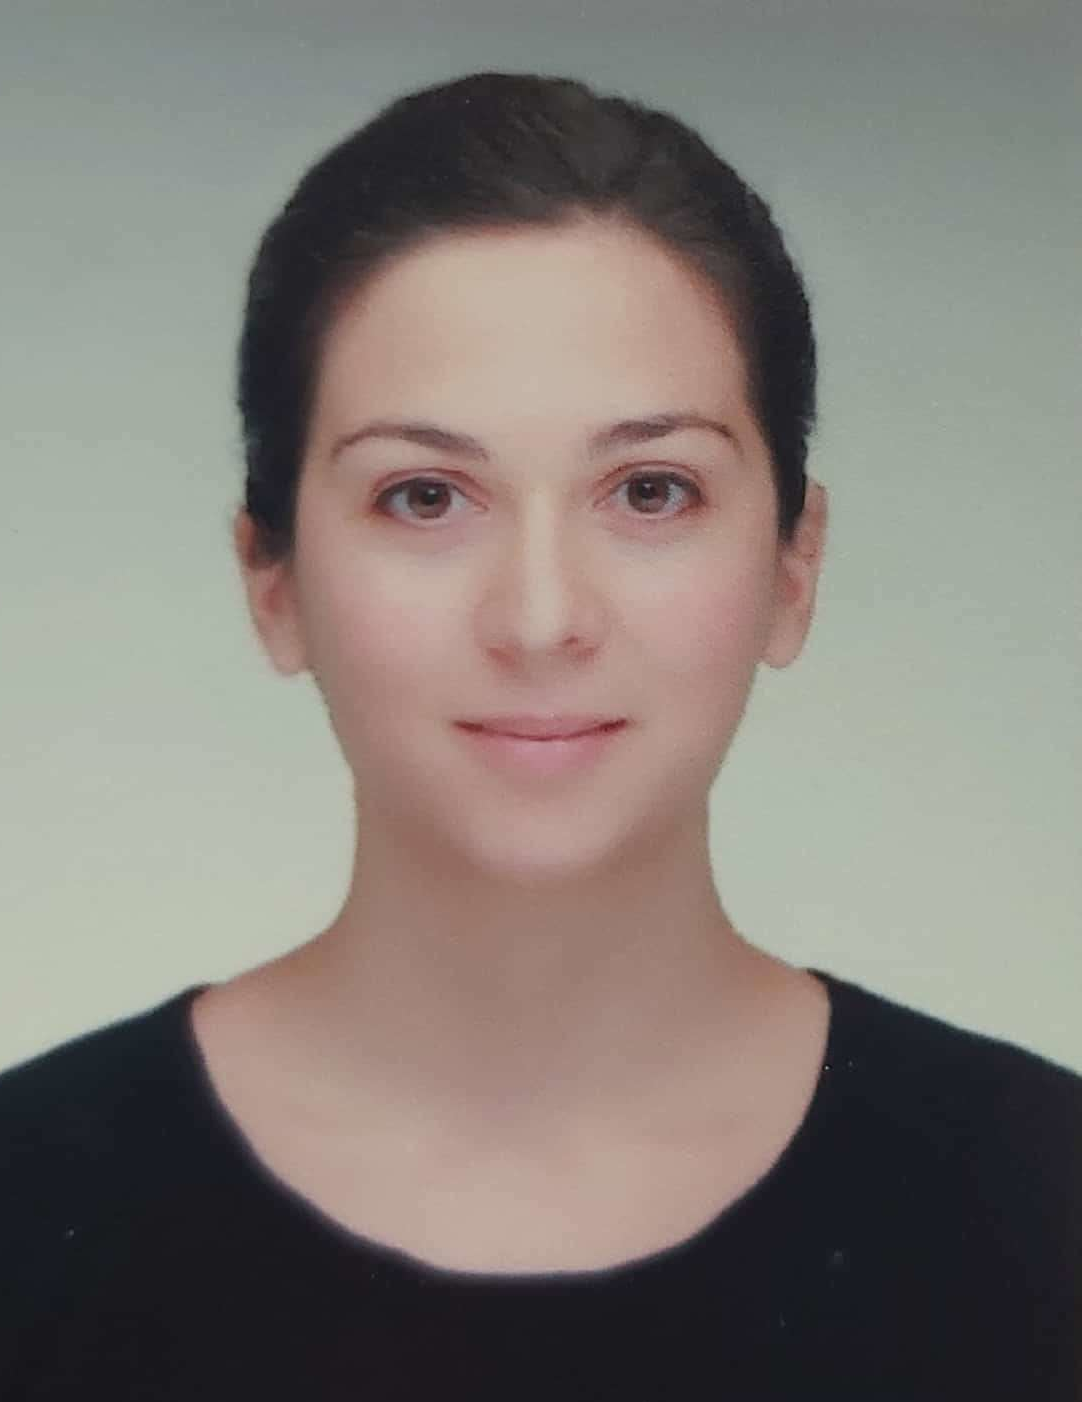
\includegraphics[width=.8\columnwidth]{img/LG}
    Disponibilité immédiate
    Permis B
    ~
    13 janvier 1989, France
    En concubinage
    %
    \section{Contact}
    laura-gomez@gmx.fr
    +33 7 70 49 23 44
    ~
    91 rue du Colonel Fabien
    92160 Antony
    France
    %
    \section{Gestion de projet}
    Microsoft Office
    ERP (Dolibarr, Sage)
    Gestion des exigences (DOORS, Reqtify)
    ~
    Rédaction brevet
    Suivi Marquage règlementaire
    Suivi de la documentation
    %
    \section{Logiciel}
    C, Matlab
    Systèmes embarqués %(Arduino, Mbed)
    CAO %(Solidworks, Fusion360, OpenSim)
    Simulation multiphysique %(Flotherm)
    Conception Electronique %(Simulink, Labview, Zuken, Altium) 
    Outils d’étude du movement humain %(Nexus pour Vicon, MT Manager pour Xsens (centrales inertielles))
    %
    \section{Langues}
    Français 
    Anglais 
    Espagnol
    %
    \section{Soft Skills}
    Autonome et proactive
    Pensée analytique
    Bon esprit d'équipe
    %
\end{aside}

\section{Rés}{umé}

Mécatronicienne de formation, j’ai eu l’occasion de piloter le développement matériel et logiciel de produits, dès leur phase de développement jusqu'à leur industrialisation ainsi que de produits déjà existants afin de les adapter aux besoins spécifiques du client.
 
Dans ce contexte, j'assure une bonne communication entre toutes les parties prenantes internes et externes concernées, afin de respecter les délais et la qualité de la prestation au client.
 
D'une grande capacité d'adaptation, j’aime apprendre au quotidien et partager mes connaissances avec mes collègues.


\section{Experience}{ Professionnelle}

\begin{entrylist}
%------------------------------------------------
\entry
  {2021}
  {NeoFarm}
  {Robotique maraichère}
  {\jobtitle{Ingénieure mécatronique -- Ingénieure industrialisation}\\
   Développements et tests d'outils maraichers adaptés au robot
   Suivi fournisseurs
   Suivi marquage réglementaire
   Mise en place ERP et règles de conception}
 
%------------------------------------------------
\entry
  {2020}
  {Safran}
  {Défense}
  {\jobtitle{Ingénieure système}\\
  Etude biomécanique

  Recueil et synthèse du besoin en provenance de diverses parties prenantes

  Recherche des solutions existantes sur le marché

  Suivi fournisseurs Français et étrangers

  Déclinaison d’exigences sous DOORS 
  }
%------------------------------------------------
\entry
  {2018--2019}
  {Safran -- Zodiac}
  {Aéronautique}
  {\jobtitle{Chef de projet technique de systèmes mécatronique}\\
  Recueil du besoin client Italien

  Traduction du besoin en actions R\&D

  Gestion des échanges technique et documentaire entre le client et les BE mécanique, logiciel et électronique

  Conception de harnais sous Zuken

  Vérification de la fabrication avec l'équipe Production

  Essais du système chez le client
 
  }
%------------------------------------------------
\entry
 {2017--2018}
 {Air Liquide Medical System}
 {Médical - ventilation}
 {\jobtitle{Référente mécanique - nouveau produit et plasturgie}\\
 En charge de l'évolution du système actuel pour réduire les fissures

 Suivi des échantillons initiaux de la coque plastique d'un nouvel appareil

 Suivi des plasturgistes

 8D et task force: Recherche, conception et réalisation d'une solution, rapidement mise en place avec l'équipe SAV
 }
%------------------------------------------------
\entry
 {2016}
 {CEA}
 {Cobotique Agro-alimentaire}
 {\jobtitle{Chef de projet technique de systèmes cobotique}\\
 Etude du besoin au poste de travail (biomécanique)

 Recherche de solutions, conception, fabrication de démonstrateurs

 Essais puis suivi de fournisseurs

 Mise en service des prototypes sur le poste de travail avec essais par les opérateurs

 Rédaction de brevets
 }
%------------------------------------------------

\end{entrylist}

%----------------------------------------------------------------------------------------
%	EDUCATION SECTION
%----------------------------------------------------------------------------------------

\section{Form}{ation}

\begin{entrylist}
%--------------------------------------G----------
\entry
{2013--2015}
{Master d'ingénierie biomédical {\normalfont spécialité biomécanique}}
{BME et Arts et Métiers}
{}
%------------------------------------------------
\entry
{2008--2013}
{Ecole d'ingénieur en mécatronique {\normalfont spécialité robotique et simulation}}
{ISTY - UVSQ}
{6 mois en Corée à l'Université Ajou}
%------------------------------------------------
% \entry
% {2003-2004}
% {Licence de chimie-physique}
% {Université Paris-Sud 11}
% {Mention TB}
% %------------------------------------------------
% \entry
% {2003-2006}
% {Magistère de Physico-Chimie Moléculaire}
% {Université Paris-Sud 11 -- ENS Cachan}
% {}
% %------------------------------------------------
% \entry
% {2001-2003}
% {CPGE {\normalfont PCSI-PC}}
% {Lycée François Arago, Perpignan}
% {}
\end{entrylist}

%----------------------------------------------------------------------------------------
%	OTHER QUALIFICATIONS SECTION
%----------------------------------------------------------------------------------------

% \section{Publications}{ significatives}

% \nocite{vallverdu2016, guille2015, Guille2014, Martin2012, Maillet2011, Vallverdu2010}
% \begin{btSect}{bib/articles}
%     \btPrintCited
% \end{btSect}

%----------------------------------------------------------------------------------------
%	INTERESTS SECTION
%----------------------------------------------------------------------------------------

% \section{Centres d'intérêts}
%   \vspace{-0.2cm}
%
% \textbf{Informatiques:} Outils numériques et pédagogiques, programmation,
% communautée open-source.\\
% \textbf{Personnels:} Membre au CA de l'association APNEE, rugby, guitare, flûte.

%----------------------------------------------------------------------------------------

\end{document}
